\clearpage
\section{Auswertung}
Die gemessenen Wertepaare der beiden Messreihen sind in Abbildung \ref{fig:Verlauf} und den
Tabellen \ref{tab:tab10} und \ref{tab:tab20} zu sehen. Es
ist zu erkennen, dass der Verlauf des Graphen für Temperaturen unter ca. $280$ K und über
ca. $310$ K ein Verhalten zeigt, dass qualitativ nicht mit dem in der Theorie erwarteten
Verhalten übereinstimmt, so dass vermutet wird, dass die Theorie nur für den entsprechenden
Bereich dazwischen gültig ist, während in den äußeren Bereichen andere Effekte berücksichtigt
werden müssen. Die gemessenen Wertepaare von Temperatur und Depolarisationsstrom sind in
Abbildung \ref{fig:Verlauf} zu sehen. Im Folgenden
beziehen sich Größen mit
Index "`1"' auf die Heizrate $b_1=2$ K/min bzw. mit Index "`2"' auf $b_2=2.5$
K/min. \\ Zunächst werden die gemessenen Daten auf den Bereich zwischen $280$ K und $310$ K
eingegrenzt durch Abschätzung des Untergrunds korrigiert.
Dazu wird der Untergrund als $j_\text{Untergrund}(T)=A\e^{B T}$ beschrieben und die Parameter
$A$ und $B$ werden über die Regressionsgerade $\ln(j_\text{Untergrund})(T)=\ln(A)+BT$ gefittet.
Da der Untergrund-Fit an einigen Stellen unter den gemessenen Werten liegt und dies ein
unphysikalisches Verhalten darstellt, wird dieser soweit
nach unten verschoben, dass er unterhalb aller Messwerte liegt.
Das Ergebnis ist in den Abbildungen \ref{fig:Messwertea}, \ref{fig:Messwerteb} und
\ref{fig:Messwertec} sowie in den Tabellen \ref{tab:tab1} und \ref{tab:tab2} zu sehen.\\ Außerdem wird in \ref{fig:Heiz} die
Heizrate gezeigt. Diese wurde als zentraler Differenzenquotient der Temperatur $T$ gemäß
\begin{equation}
b_t=\frac{T_{t+1}-T_{t-1}}{2 \text{min}}
\end{equation}
berechnet. Dabei ist zu erwähnen, dass die in Tabelle \ref{tab:tab1} und \ref{tab:tab2} zu
sehenden Messwerte in Zeitabständen von einer Minute gemessen wurden. Im Durchschnitt ergeben
sich so als reale Heizraten
\begin{align}
b_{1,\text{real}}&=( 1.63 \pm 0.31 ) \text{ K/min}\\
b_{2,\text{real}}&= (2.41 \pm 0.30 ) \text{ K/min} \quad .
\end{align}


\begin{figure}[t]
\centering
\includegraphics[scale=0.8]{../skript/Heizrate.pdf}
\caption{Heizrate der zwei Messreihen.}
\label{fig:Heiz}
\end{figure}

\begin{figure}
\centering
\includegraphics[scale=0.8]{../skript/Temp_Strom_Verlauf0.pdf}
\caption{Temperatur-Strom-Verlauf der zwei Messreihen.}
\label{fig:Verlauf}
\end{figure}




\begin{figure}[H]
\centering
\includegraphics[scale=0.8]{../skript/Temp_Strom_Verlaufa.pdf}
\caption{Gemessener Temperatur-Strom-Verlauf und Untergrundabschätzung für die erste Messung.}
\label{fig:Messwertea}
\includegraphics[scale=0.8]{../skript/Temp_Strom_Verlaufb.pdf}
\caption{Gemessener Temperatur-Strom-Verlauf und Untergrundabschätzung für die zweite Messung.}
\label{fig:Messwerteb}
\end{figure}
\begin{figure}
\centering
\includegraphics[scale=0.8]{../skript/Temp_Strom_Verlaufc.pdf}
\caption{Korrigierter Temperatur-Strom-Verlauf.}
\label{fig:Messwertec}
\end{figure}

\begin{table}[htpb]
	\centering
	\begin{tabular}{cc|cc|cc}
		\midrule
		\midrule
		$T / \si{\kelvin}$ &
		$I / \si{\pA}$ &
		$T / \si{\kelvin}$ &
		$I / \si{\pA}$ &
		$T / \si{\kelvin}$ &
		$I / \si{\pA}$ \\
		\midrule
		233.1             & 0.60              & 272.6             & 0.37              & 318.9             & 2.55             \\
234.9             & 0.50              & 274.1             & 0.38              & 320.9             & 3.00             \\
236.6             & 0.46              & 275.3             & 0.39              & 324.1             & 3.80             \\
238.3             & 0.44              & 276.8             & 0.40              & 325.9             & 3.40             \\
239.9             & 0.41              & 278.4             & 0.43              & 327.8             & 5.00             \\
241.6             & 0.40              & 280.1             & 0.47              & 329.3             & 5.50             \\
243.3             & 0.39              & 281.8             & 0.50              & 332.5             & 6.70             \\
244.9             & 0.37              & 283.4             & 0.60              & 333.9             & 7.40             \\
246.5             & 0.35              & 285.2             & 0.75              & 335.8             & 7.90             \\
248.3             & 0.33              & 287.1             & 0.89              & 336.8             & 8.20             \\
249.6             & 0.34              & 289.1             & 1.10              & 338.3             & 8.60             \\
251.1             & 0.33              & 291.1             & 1.20              & 339.9             & 8.90             \\
252.6             & 0.32              & 293.1             & 1.20              & 341.6             & 9.00             \\
254.0             & 0.32              & 294.8             & 1.20              & 343.4             & 9.00             \\
255.5             & 0.32              & 296.6             & 1.15              & 345.1             & 9.00             \\
256.9             & 0.32              & 298.5             & 1.10              & 346.9             & 8.80             \\
258.8             & 0.32              & 301.8             & 1.15              & 348.5             & 8.60             \\
259.8             & 0.31              & 303.5             & 1.20              & 350.1             & 8.50             \\
261.1             & 0.32              & 304.9             & 1.25              & 351.8             & 8.30             \\
262.6             & 0.32              & 306.4             & 1.30              & 353.2             & 8.20             \\
263.8             & 0.32              & 307.8             & 1.35              & 354.8             & 8.00             \\
264.9             & 0.33              & 309.3             & 1.45              & 356.1             & 7.90             \\
266.2             & 0.34              & 310.9             & 1.55              & 357.4             & 7.80             \\
267.5             & 0.34              & 312.6             & 1.70              & 358.8             & 7.70             \\
268.8             & 0.35              & 314.2             & 1.85              & 360.1             & 7.50             \\
270.1             & 0.35              & 315.9             & 2.10              & -                 & -                \\
271.4             & 0.36              & 317.4             & 2.30              & -                 & -                \\
		\midrule
		\midrule
	\end{tabular}
	\caption{Gemessene Ströme $I$ in Abhängigkeit der Temperatur $T$ mit
		einer Heizrate von $b_1 = \SI{2}{\kelvin\per\minute}$.}
	\label{tab:tab10}
\end{table}
%
\begin{table}[htpb]
	\centering
	\begin{tabular}{cc|cc|cc}
		\midrule
		\midrule
		$T / \si{\kelvin}$ &
		$I / \si{\pA}$ &
		$T / \si{\kelvin}$ &
		$I / \si{\pA}$ &
		$T / \si{\kelvin}$ &
		$I / \si{\pA}$ \\
		\midrule
		233.1             & 0.60              & 278.3             & 0.45              & 323.9             & \phantom{0}2.50  \\
235.5             & 0.53              & 281.0             & 0.47              & 326.3             & \phantom{0}2.85  \\
238.1             & 0.49              & 283.1             & 0.55              & 328.8             & \phantom{0}3.40  \\
240.7             & 0.47              & 285.1             & 0.66              & 331.4             & \phantom{0}4.10  \\
243.3             & 0.44              & 287.3             & 0.89              & 333.6             & \phantom{0}4.70  \\
245.9             & 0.42              & 289.9             & 1.20              & 335.9             & \phantom{0}5.50  \\
248.5             & 0.40              & 292.4             & 1.60              & 338.4             & \phantom{0}6.40  \\
251.0             & 0.40              & 294.9             & 1.90              & 341.0             & \phantom{0}7.20  \\
253.5             & 0.39              & 299.9             & 1.75              & 343.5             & \phantom{0}8.10  \\
255.8             & 0.39              & 300.4             & 1.50              & 346.0             & \phantom{0}9.10  \\
258.1             & 0.39              & 302.3             & 1.40              & 348.5             & \phantom{0}9.90  \\
260.3             & 0.38              & 304.6             & 1.40              & 350.9             & 10.50            \\
262.3             & 0.38              & 306.8             & 1.35              & 353.1             & 11.00            \\
265.1             & 0.40              & 309.0             & 1.45              & 355.4             & 11.00            \\
267.0             & 0.40              & 311.3             & 1.50              & 357.8             & 11.00            \\
269.1             & 0.40              & 313.5             & 1.60              & 360.3             & 10.50            \\
271.1             & 0.41              & 316.2             & 1.80              & 363.1             & 10.00            \\
273.4             & 0.42              & 318.6             & 1.95              & 365.6             & \phantom{0}9.90  \\
276.1             & 0.43              & 321.3             & 2.20              & 368.6             & \phantom{0}9.70  \\
		\midrule
		\midrule
	\end{tabular}
	\caption{Gemessene Ströme $I$ in Abhängigkeit der Temperatur $T$ mit
		einer Heizrate von $b_2 = \SI{2.5}{\kelvin\per\minute}$.}
	\label{tab:tab20}
\end{table}


\begin{table}[htpb]
	\centering
	\begin{tabular}{cc|cc|cc}
		\midrule
		\midrule
		$T / \si{\kelvin}$ &
		$I / \si{\pA}$ &
		$T / \si{\kelvin}$ &
		$I / \si{\pA}$ &
		$T / \si{\kelvin}$ &
		$I / \si{\pA}$ \\
		\midrule
		# T/°C 	I/A 	I_H/A
-40 	0.06e-11 	0.8
-38.2 	0.05e-11 	0.8
-36.5 	0.046e-11  	0.8
-34.8 	0.044e-11  	0.9
-33.2 	0.041e-11 	0.9
-31.5 	0.040e-11 	0.9
-29.8 	0.039e-11 	1.0
-28.2 	0.037e-11 	1.0
-26.6 	0.035e-11 	1.0
-24.8 	0.033e-11 	1.0
-23.5 	0.034e-11 	1.0
-22.0 	0.033e-11 	1.0
-20.5 	0.032e-11 	1.0
-19.1 	0.032e-11 	1.2
-17.6 	0.032e-11 	1.2
-16.2 	0.032e-11 	1.2
-14.3 	0.032e-11 	1.2
-13.4 	0.031e-11 	1.2
-12.0 	0.032e-11 	1.2
-10.5 	0.032e-11 	1.3
-9.4 	0.032e-11 	1.4
-8.2 	0.033e-11 	1.4
-6.9 	0.034e-11 	1.4
-5.6 	0.034e-11 	1.4
-4.3 	0.035e-11 	1.5
-3.0 	0.035e-11 	1.5
-1.7 	0.036e-11 	1.7
-0.5 	0.037e-11 	1.7
1.0 	0.038e-11 	1.7
2.2 	0.039e-11 	1.7
3.7 	0.040e-11 	2.0
5.3 	0.043e-11 	2.0
7.0 	0.047e-11 	2.0
8.6 	0.050e-11 	2.0
10.3 	0.060e-11 	2.2
12.1 	0.075e-11 	2.3
14.0 	0.089e-11 	2.3
16.0 	0.110e-11 	2.3
18.0 	0.120e-11 	2.3
20.0 	0.120e-11 	2.3
21.7 	0.120e-11 	2.3
23.5 	0.115e-11 	2.3
25.4 	0.110e-11 	2.3
28.6 	0.115e-11 	2.3
30.4 	0.120e-11 	2.3
31.8 	0.125e-11 	2.3
33.3 	0.130e-11 	2.3
34.7 	0.135e-11 	2.3
36.2 	0.145e-11 	2.5
37.8 	0.155e-11 	2.5
39.5 	0.170e-11 	2.5
41.1 	0.185e-11 	2.5
42.8 	0.210e-11 	2.5
44.3 	0.230e-11 	2.5
45.8 	0.255e-11 	2.7
47.8 	0.300e-11 	2.7
51.0 	0.38e-11 	2.7
52.8 	0.34e-11 	2.7
54.6 	0.50e-11 	2.7
56.2 	0.55e-11 	2.7
59.4 	0.67e-11 	2.7
60.8 	0.74e-11 	2.7
62.7 	0.79e-11 	2.7
63.7 	0.82e-11 	2.7
65.2 	0.86e-11 	2.7
66.8 	0.89e-11 	2.9
68.5 	0.90e-11 	2.9
70.3 	0.90e-11 	2.9
72.0 	0.90e-11 	2.9
73.8 	0.88e-11 	2.9
75.4 	0.86e-11 	2.9
77.0 	0.85e-11 	2.9
78.7 	0.83e-11 	2.9
80.1 	0.82e-11 	2.9
81.6 	0.80e-11 	2.9
83.0 	0.79e-11 	2.9
84.3 	0.78e-11 	2.9
85.7 	0.77e-11 	2.9
87.0 	0.75e-11 	2.9

		\midrule
		\midrule
	\end{tabular}
	\caption{Korrigierte Ströme $I$ in Abhängigkeit der Temperatur $T$ mit
		einer Heizrate von $b_1 = \SI{2}{\kelvin\per\minute}$.}
	\label{tab:tab1}
\end{table}
%
\begin{table}[htpb]
	\centering
	\begin{tabular}{cc|cc|cc}
		\midrule
		\midrule
		$T / \si{\kelvin}$ &
		$I / \si{\pA}$ &
		$T / \si{\kelvin}$ &
		$I / \si{\pA}$ &
		$T / \si{\kelvin}$ &
		$I / \si{\pA}$ \\
		\midrule
		# T/°C 	I/A 	I_H/A
-40.0 	0.060e-11 	1.5
-37.6 	0.053e-11 	1.5
-35.0 	0.049e-11 	1.5
-32.4 	0.047e-11 	1.5
-29.8 	0.044e-11 	1.7
-27.2 	0.042e-11 	1.7
-24.6 	0.040e-11 	1.7
-22.1 	0.040e-11 	1.7
-19.6 	0.039e-11 	1.7
-17.3 	0.039e-11 	1.7
-15.0 	0.039e-11 	1.7
-12.8 	0.038e-11 	1.7
-10.8 	0.038e-11 	2.0
-8.0 	0.040e-11 	2.0
-6.1 	0.040e-11 	2.0
-4.0 	0.040e-11 	2.0
-2.0 	0.041e-11 	2.3
0.3 	0.042e-11 	2.3
3.0 	0.043e-11 	2.3
5.2 	0.045e-11 	2.3
7.9 	0.047e-11 	2.3
10.0 	0.055e-11 	2.3
12.0 	0.066e-11 	2.3
14.2 	0.089e-11 	2.6
16.8 	0.120e-11 	2.6
19.3 	0.160e-11 	2.6
21.8 	0.190e-11 	2.6
27.3 	0.175e-11 	2.6
26.8 	0.150e-11 	2.6
29.2 	0.140e-11 	2.6
31.5 	0.140e-11 	2.6
33.6 	0.135e-11 	2.6
35.9 	0.145e-11 	2.8
38.2 	0.150e-11 	2.8
40.4 	0.160e-11 	2.8
43.1 	0.180e-11 	3.0
45.5 	0.195e-11 	3.0
48.2 	0.220e-11 	3.0
50.8 	0.250e-11 	3.0
53.2 	0.285e-11 	3.0
55.7 	0.340e-11 	3.0
58.3 	0.410e-11 	3.0
60.5 	0.470e-11 	3.0
62.8 	0.550e-11 	3.0
65.3 	0.640e-11 	3.2
67.9 	0.720e-11 	3.2
70.4 	0.810e-11 	3.2
72.9 	0.910e-11 	3.2
75.4 	0.990e-11 	3.2
77.8 	1.05e-11 	3.2
80.0 	1.10e-11 	3.2
82.3 	1.10e-11 	3.2
84.6 	1.10e-11 	3.2
87.2 	1.05e-11 	3.2
90.0 	1.00e-11 	3.2
92.5 	0.99e-11 	3.2
95.5 	0.97e-11 	3.2

		\midrule
		\midrule
	\end{tabular}
	\caption{Korrigierte Ströme $I$ in Abhängigkeit der Temperatur $T$ mit
		einer Heizrate von $b_2 = \SI{2.5}{\kelvin\per\minute}$.}
	\label{tab:tab2}
\end{table}
%
\clearpage
\subsection{Bestimmung von $W$ aus dem ersten Teil des Kurvenverlaufes}
Für Temperaturen nahe bei $T_0:=\min\{T_1\}$ gilt die Abhängigkeit
\begin{equation}
j(T)\propto \text{e}^{-W/\text{k}_\text{B}T} \quad ,
\end{equation}
wobei $j$ der Depolarisationsstrom, $W$ die Aktivierungsenergie, $T$ die
Temperatur sind, sowie $\text{e}$ und $\text{k}_\text{B}$ die Eulersche- und
Boltzmannkonstanten.

Ein linearer Fit für $\ln(j)$ gegen $1/T$ ergibt
%\input{G1}
%\input{G2}
\begin{align}
G_1(x)&= -( 26.1\pm 4.3)\times 10^{3} \,x - (62 \pm 15) \\
G_2(x)&= -(27.3 \pm 3.1 )\times 10^{3} \,x - (65 \pm 10)
\end{align}
Die Graphen dazu sind in den Abbildungen \ref{fig:G1} und \ref{fig:G2} zu sehen.

\begin{figure}[h]
\centering
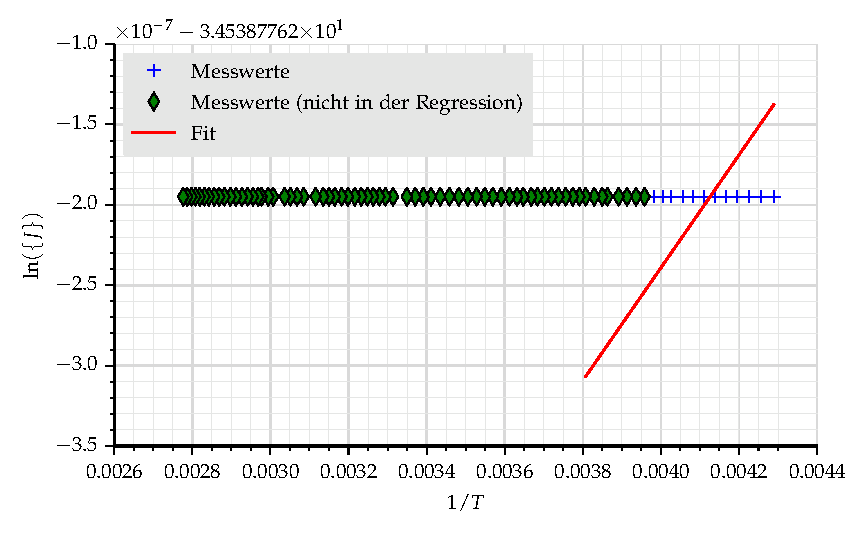
\includegraphics[scale=0.8]{../skript/G1.pdf}
\caption{Darstellung der Messwerte zur Heizrate $b=2.0$ K/min.}
\label{fig:G1}
\end{figure}
\begin{figure}[h]
\centering
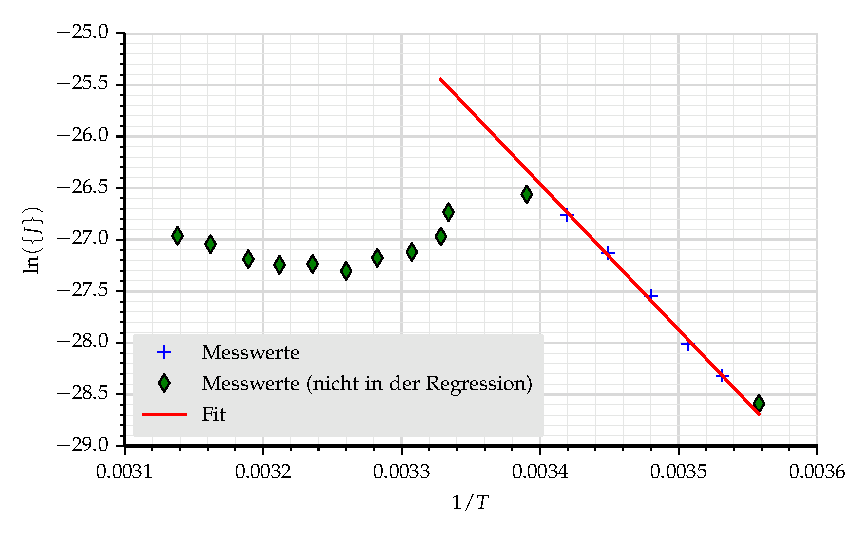
\includegraphics[scale=0.8]{../skript/G2.pdf}
\caption{Darstellung der Messwerte zur Heizrate $b=2.5$ K/min.}
\label{fig:G2}
\end{figure}



Damit ergibt sich
\begin{align}
W_1&= (3.61 \pm 0.59)\times 10^{-19}\text{J}=(2.25 \pm 0.37)\text{ eV}\\
W_2&=  (3.77 \pm 0.43) \times 10^{-19}\text{J}=(2.35 \pm 0.26)\text{ eV}\quad .
\end{align}
Da bei der Rechnung nur eine fehlerbehaftete Größe (die Steigung der
Ausgleichsgeraden) vorkommt, sind die Fehlerrechnung identisch mit der
zum Mittelwert.
\subsection{Bestimmung von $W$ aus dem gesamten Kurvenverlauf}
Definiere
\begin{equation}
S(T)=\int\limits_T^{T^*} j(T') \text{d}T' \frac{1}{j(T)} \label{eq:s}
\end{equation}
mit dem letzten gemessenen Wert $T^*$\footnote{Für die erste Messreihe war dies $310$ K, für
die zweite Messreihe $320$ K.}. Statt des Stroms $i$ kann hier die
Stromdichte $j$ benutzt werden, da sich $i$ und $j$ nur um einen Faktor (
Querschnittsfläche des Kabels) unterscheiden, und dieser bei der weiteren
Berechnung wegfällt.
Bei konstanter Heizrate gilt
\begin{equation}
\frac{W}{\text{k}_\text{B} T}=\ln S(T)
\end{equation}
mit einer Konstanten $k$. Bei der Berechnung wurde die Näherung
\begin{equation}
S(T)=\int\limits_T^{T^*} j(T') \text{d}T' \approx \sum\limits_{\#\text{Messwerte}} j^n  \hat{b}
\end{equation}
benutzt. Der Index bezieht sich dabei auf den $n$-ten Messwert, $\hat{b}$ ist die
Heizrate in SI-Einheiten.\\
Die so ermittelten Werte sind in den Tabellen \ref{tab:3} und \ref{tab:4} zu sehen. Die
sehr großen $S$ Werte für kleine $T$ liegen an der $1/j(T)$-Abhängigkeit in $S$ (vgl.
\eqref{eq:s}),
und dem Umstand, dass der Untergrund-Fit gerade so angepasst wurde, dass der Strom $j(T)$ für
kleine $T$ nahe null liegt.

\begin{table}
\centering
\begin{tabular}{cccccc}
\toprule
\midrule
$T$ & $S(T)$&$T$ & $S(T)$&$T$ & $S(T)$ \\
\midrule
280.1             & 575230078.61      & 291.1             & 7.95              & 303.5             & \phantom{0}5.24  \\
281.8             & \phantom{0000}71341.50 & 293.1             & 6.74              & 304.9             & \phantom{0}4.20  \\
283.4             & \phantom{0000000}86.78 & 294.8             & 5.39              & 306.4             & \phantom{0}4.37  \\
285.2             & \phantom{0000000}31.55 & 296.6             & 4.77              & 307.8             & 34.70            \\
287.1             & \phantom{0000000}19.15 & 298.5             & 4.89              & 309.3             & \phantom{0}2.00  \\
289.1             & \phantom{0000000}10.81 & 301.8             & 5.55              & -                 & -                \\
\midrule
\bottomrule
\end{tabular}
\caption{Die ermittelten $S$ Werte für die erste Messreihe.}
\label{tab:3}
\end{table}

\begin{table}
\centering
\begin{tabular}{cccccc}
\toprule
\midrule
$T$ & $S(T)$&$T$ & $S(T)$&$T$ & $S(T)$ \\
\midrule
281.0             & 1350352945.62     & 294.9             & \phantom{0}8.06   & 309.0             & \phantom{0}8.14  \\
283.1             & \phantom{0000000}340.74 & 299.9             & \phantom{0}7.74   & 311.3             & 11.77            \\
285.1             & \phantom{0000000}123.59 & 300.4             & \phantom{0}7.92   & 313.5             & 12.93            \\
287.3             & \phantom{00000000}45.30 & 302.3             & \phantom{0}8.02   & 316.2             & \phantom{0}5.00  \\
289.9             & \phantom{00000000}23.08 & 304.6             & \phantom{0}7.41   & 318.6             & \phantom{0}2.50  \\
292.4             & \phantom{00000000}12.68 & 306.8             & 10.34             & -                 & -                \\
\midrule
\bottomrule
\end{tabular}
\caption{Die ermittelten $S$ Werte für die zweite Messreihe.}
\label{tab:4}
\end{table}


 Ein linearer Fit für $\ln(S(T))$ gegen $1/T$ ergibt
%\input{GS1}
%\input{GS2}
\begin{align}
G_{S,1}(x)&= (8.8 \pm 1.6 )\times 10^{3} \,x - (27.9 \pm 5.5)  \\
G_{S,2}(x)&= (5.6 \pm 1.7 )\times 10^{3} \,x - (16.1 \pm 5.8)
\end{align}
Die entsprechenden Abbildungen sind \ref{fig:GS1} und \ref{fig:GS2}.
\begin{figure}[h]
\centering
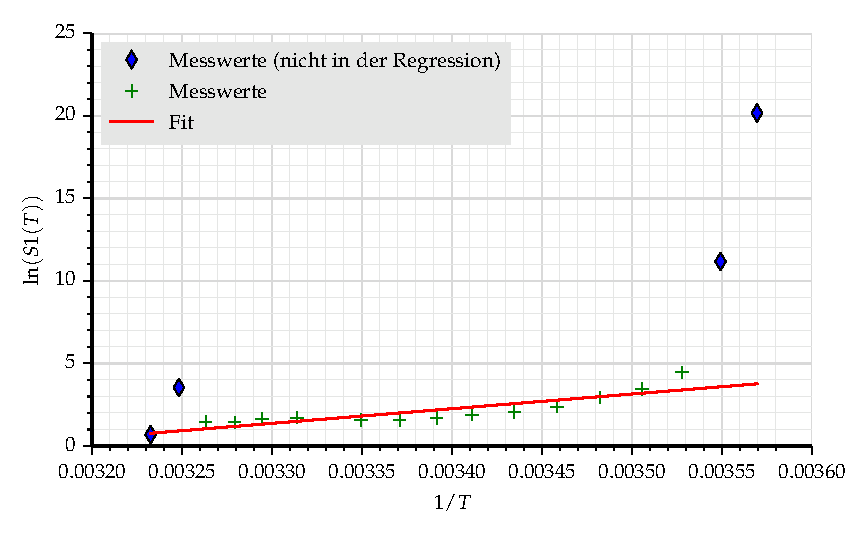
\includegraphics[scale=0.8]{../skript/S1.pdf}
\caption{Darstellung der Messwerte zur Heizrate $b=2.0$ K/min.}
\label{fig:GS1}
\end{figure}
\begin{figure}[h]
\centering
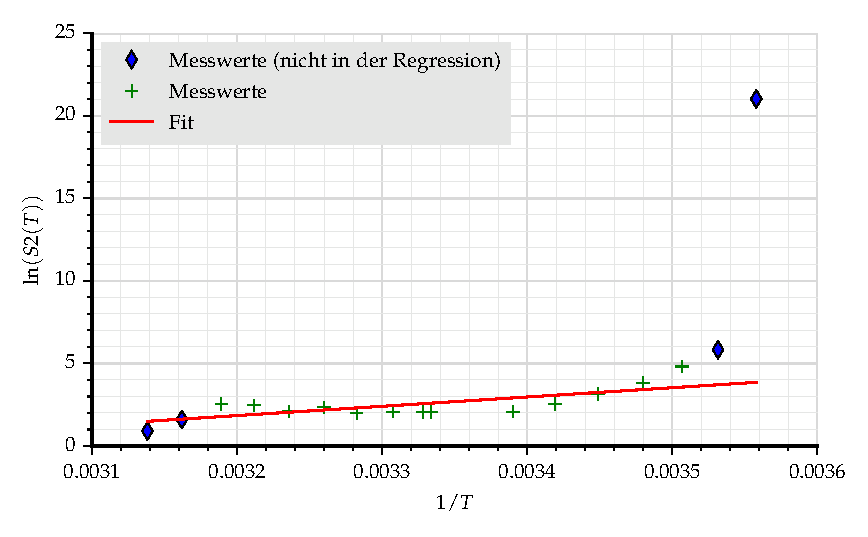
\includegraphics[scale=0.8]{../skript/S2.pdf}
\caption{Darstellung der Messwerte zur Heizrate $b=2.5$ K/min.}
\label{fig:GS2}
\end{figure}
Es folgen
\begin{align}
W_{S,1}&=  (1.22 \pm 0.22)\times 10^{-19}\text{ J} = (0.76\pm 0.13)\text{ eV} \label{W1} \\
W_{S,2}&=  (7.77 \pm 2.43) \times 10^{-20}\text{ J} = (0.48\pm 0.15)\text{ eV}\quad . \label{W2}
\end{align}
Da wieder nur eine fehlerbehaftete Größe vorkommt, kann der Fehler wie der
Messwert behandelt werden.


\subsection{Bestimmung der Relaxationszeit $\tau$}
Differentiation von Gleichung \eqref{eq:Stromdichte} ergibt
\begin{equation}
\frac{1}{b}+ \frac{\text{d}}{\text{d}T}\eval_\text{max}\tau(T)=0
\end{equation}
mit $T_\text{max}=\max\{T \}$. Mit
\begin{equation}
 \frac{\text{d}}{\text{d}T}\eval_\text{max}\tau(T) =-\frac{W}{\text{k}_\text{B}
 T^2}
\end{equation}
folgt
\begin{equation}
\tau(T_\text{max})=\frac{\text{k}_\text{B} T_\text{max}^2}{W b} \quad . \label{eq:taumax}
\end{equation}
Nun kann mit Hilfe von Gleichung \eqref{eq:relaxationszeit} die Relaxationszeit $\tau_0$
gemäß
\begin{equation}
\tau_0=\tau(T_\text{max})\text{e}^{-\frac{W}{\text{k}_\text{B}T_\text{max}}} \label{eq:tau0}
\end{equation}
bestimmt werden.

So ergibt sich
\begin{align}
\tau_{0,1} &=(0.26 \pm 1.50)\times
10^{-12} \text{ s} \\
\tau_{0,2} &=(0.32\pm 1.91)\times
10^{-7} \text{ s}
\end{align}

Die Fehlerrechnung geschieht dabei mit gemäß der Gaußschen Fehlerfortpflanzung:\\
Mit \eqref{eq:taumax} in \eqref{eq:tau0} und der Gaußschen Fehlerfortplanzung
\begin{equation}
\Delta \tau_0=\sqrt{\left(\frac{\partial \tau_0}{\partial W} \, \Delta W \right)^2} \quad ,
\end{equation}
wobei $\Delta \tau_0$ den erwarteten Fehler von $\tau_0$ und $\Delta W$ den erwarteten Fehler
von $W$ darstellen, ergibt sich
\begin{align}
\Delta \tau_0=\left| -\frac{\kB T_\text{max}^2}{W^2 b} \e^{-\frac{W}{\kB T_\text{max}}} - \frac{
\kB T^2_\text{max}}{Wb}\frac{1}{\kB T_\text{max}} \e^{-\frac{W}{\kB T}} \right|\Delta W
\end{align}
wobei für $W$ und $\Delta W$ jeweils die Werte aus \eqref{W1} und \eqref{W2} eingesetzt wurden
und $b$ entsprechend die Heizrate $b_1$ bzw. $b_2$ ist.
\clearpage
